\documentclass[12pt, letterpaper]{article}
\usepackage{graphicx}
\usepackage{amsmath}% For the equation* environment
\title{运用贝叶斯模型计算恒星速度弥散}
\PassOptionsToPackage{quiet}{fontspec}
\usepackage[UTF8]{ctex}
\author{Suiran}
\begin{document}
\maketitle

\newpage
\section{单参数模型}
\subsection{模型}
在Lamost网站[http://www.lamost.org/public/],从北天极附近的20个平方度内下载数据。

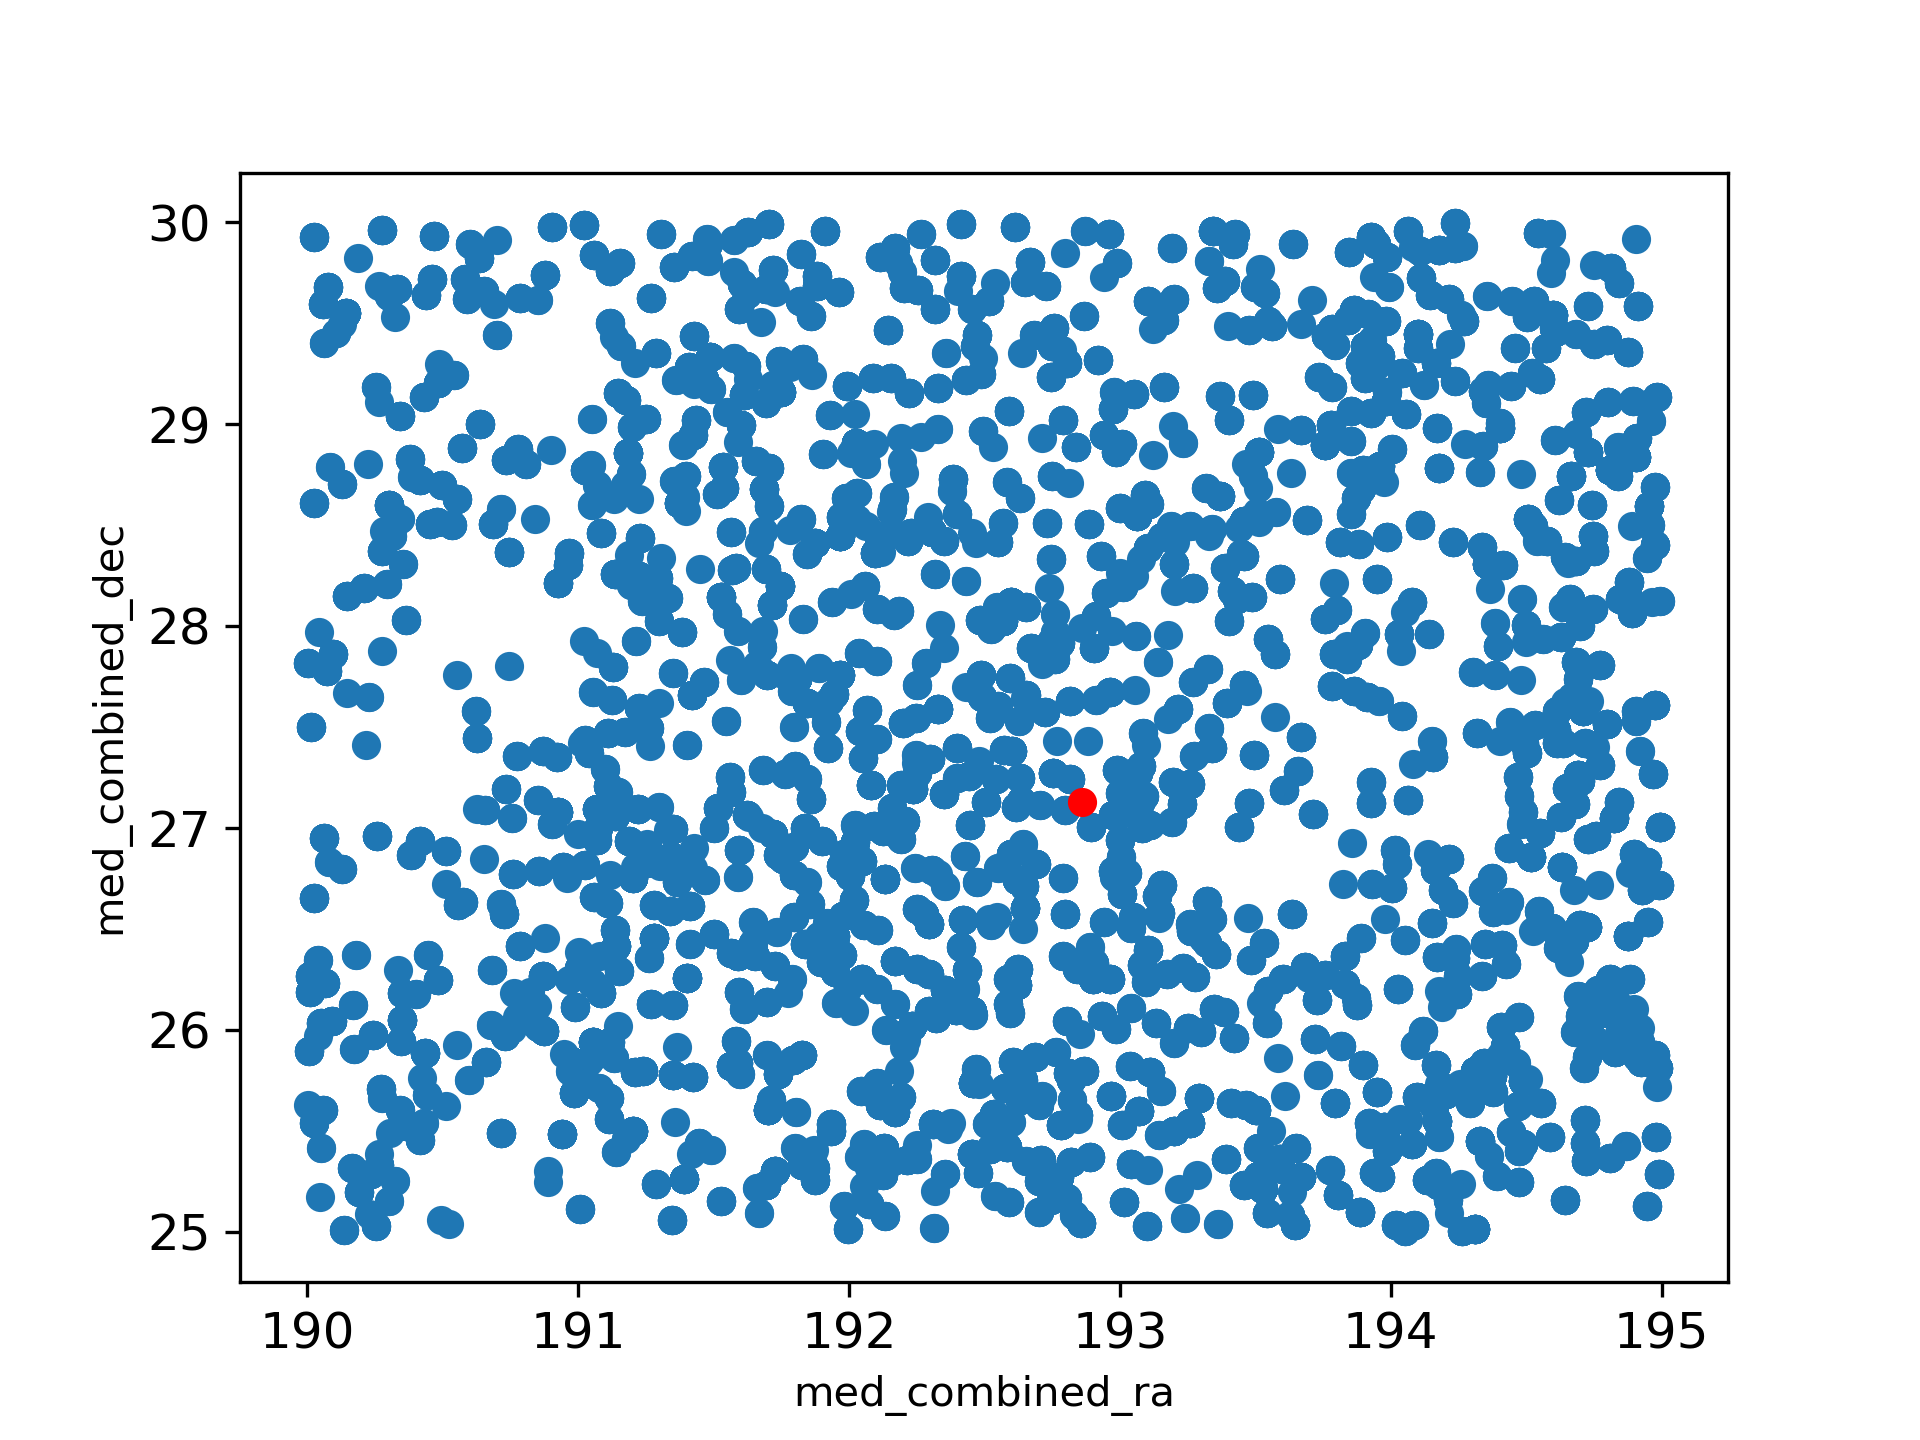
\includegraphics[scale=0.7]{3_0.png}

根据样本数据,猜测恒星的视向速度满足正态分布,似然分布为:
$$\begin{aligned}
p(y|\sigma^2)&\propto \sigma^{-n}\exp\left(-\frac{1}{2\sigma^2}\sum^{n}_{i=1}(y_i-\theta)^2\right) \\
&=(\sigma^2)^{-\frac{n}{2}}e^{\frac{n}{2\sigma^2}v^2} 
\end{aligned}
$$
由于正态分布的共轭先验分布为逆伽玛分布,故可以假定先验分布的形式为:
$$p(\sigma^2)\propto(\sigma^2)^{-(\alpha+1)}e^{-\beta/\sigma^2}$$
其中$\alpha,\beta$为先验的超参数,我们可以根据经验获取先验分布的$\sigma$值,从而求得超参数$\alpha,\beta$。
对于$\sigma$的值,我们取为20,根据伽玛分布的期望、方差和超参数的关系$\sigma^2_0=\frac{\beta}{\alpha-1},[\sigma_0^2-(\sigma_0-10)^2]^2=\frac{\beta^2}{(\alpha-1)^2(\alpha-2)}$,可以近似的求出超参数。
由以上先验分布和似然分布可以得后验分布:
$$p(\sigma^2|y)\propto p(y|\sigma^2)p(\sigma^2)=(\sigma^2)^{-(\alpha+\frac n2+1)}\exp{-\frac 1\sigma^2(\frac{nv^2}{2}+\beta)}$$
即$\sigma^2|y$也服从逆伽马分布,其参数为$(\alpha^{\prime}=\alpha+\frac n2,\beta^{\prime}=\frac{nv^2}{2}+\beta)$。
\subsection{程序}
另附
\subsection{结果}
区域星体速度弥散的平方为$\sigma^2=914.8km^2/s^2$

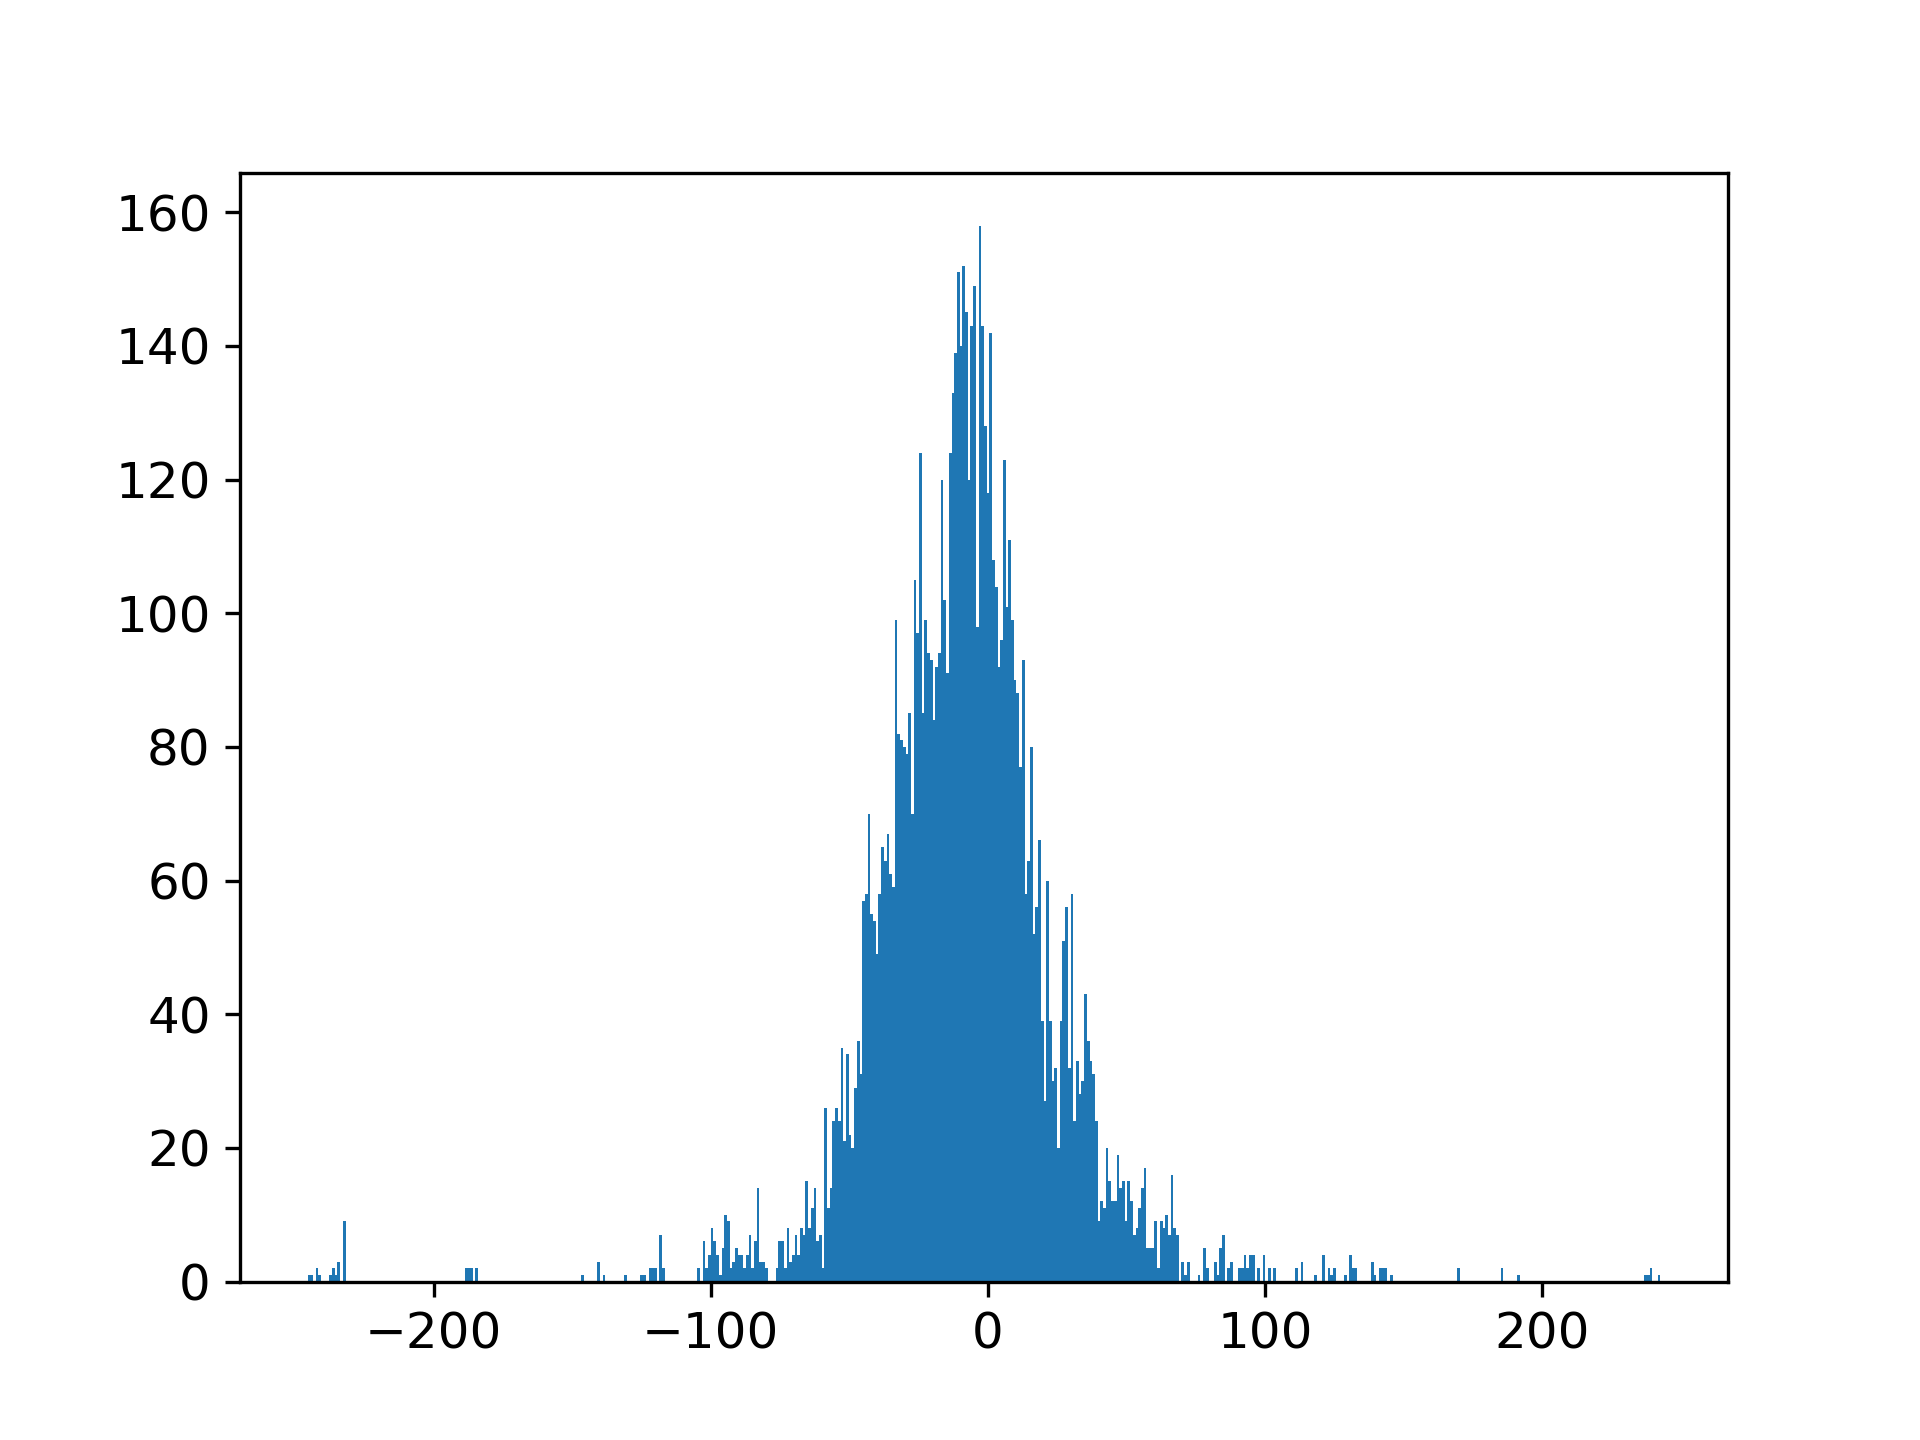
\includegraphics[scale=0.7]{3_1.png}

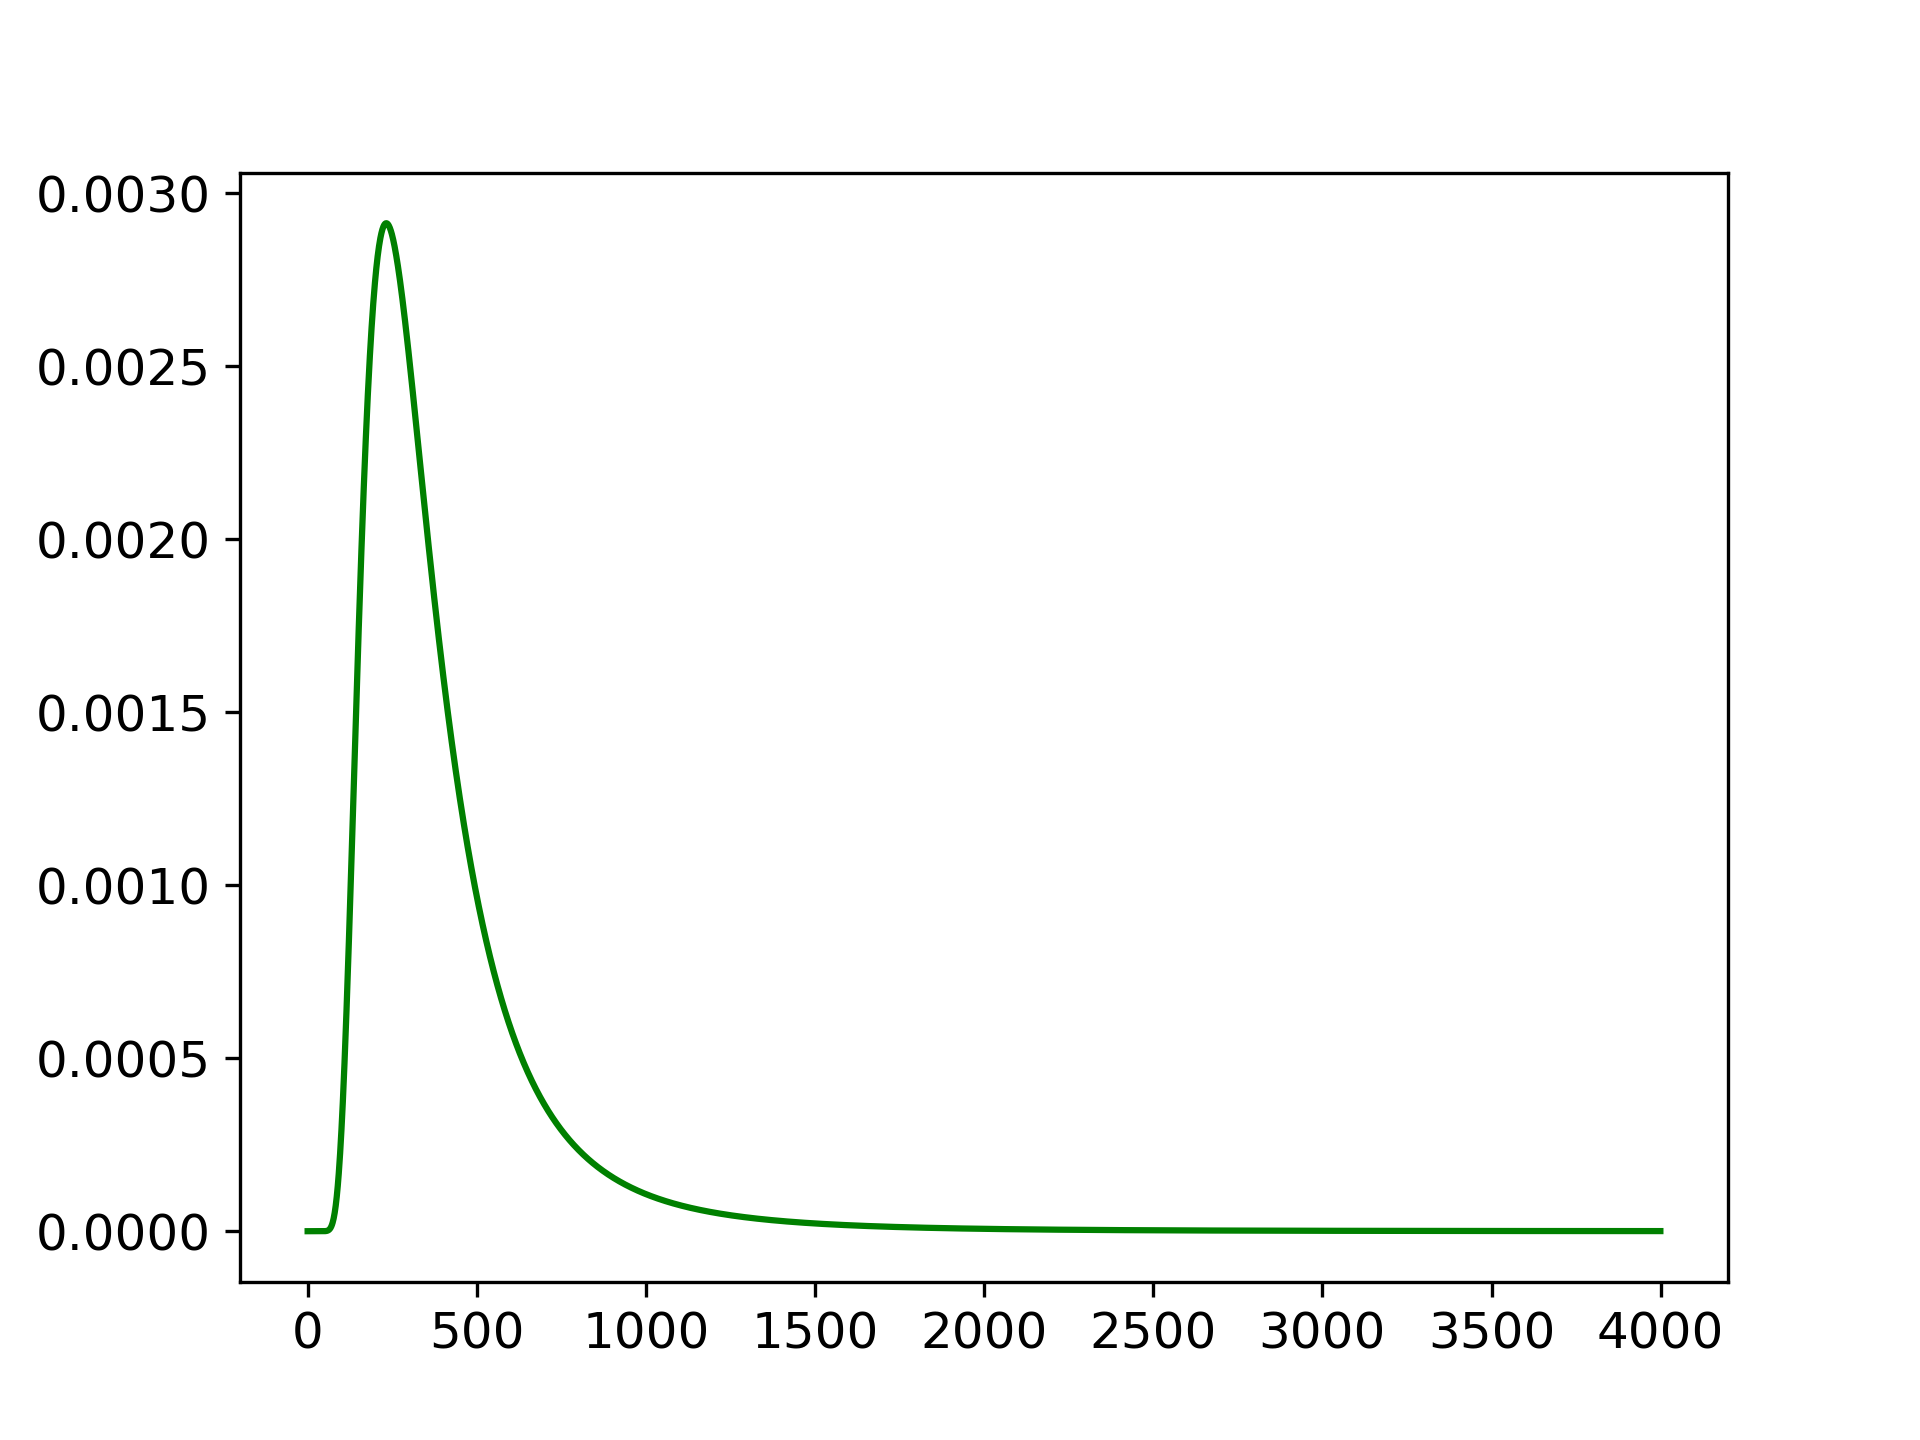
\includegraphics[scale=0.7]{3_2.png}

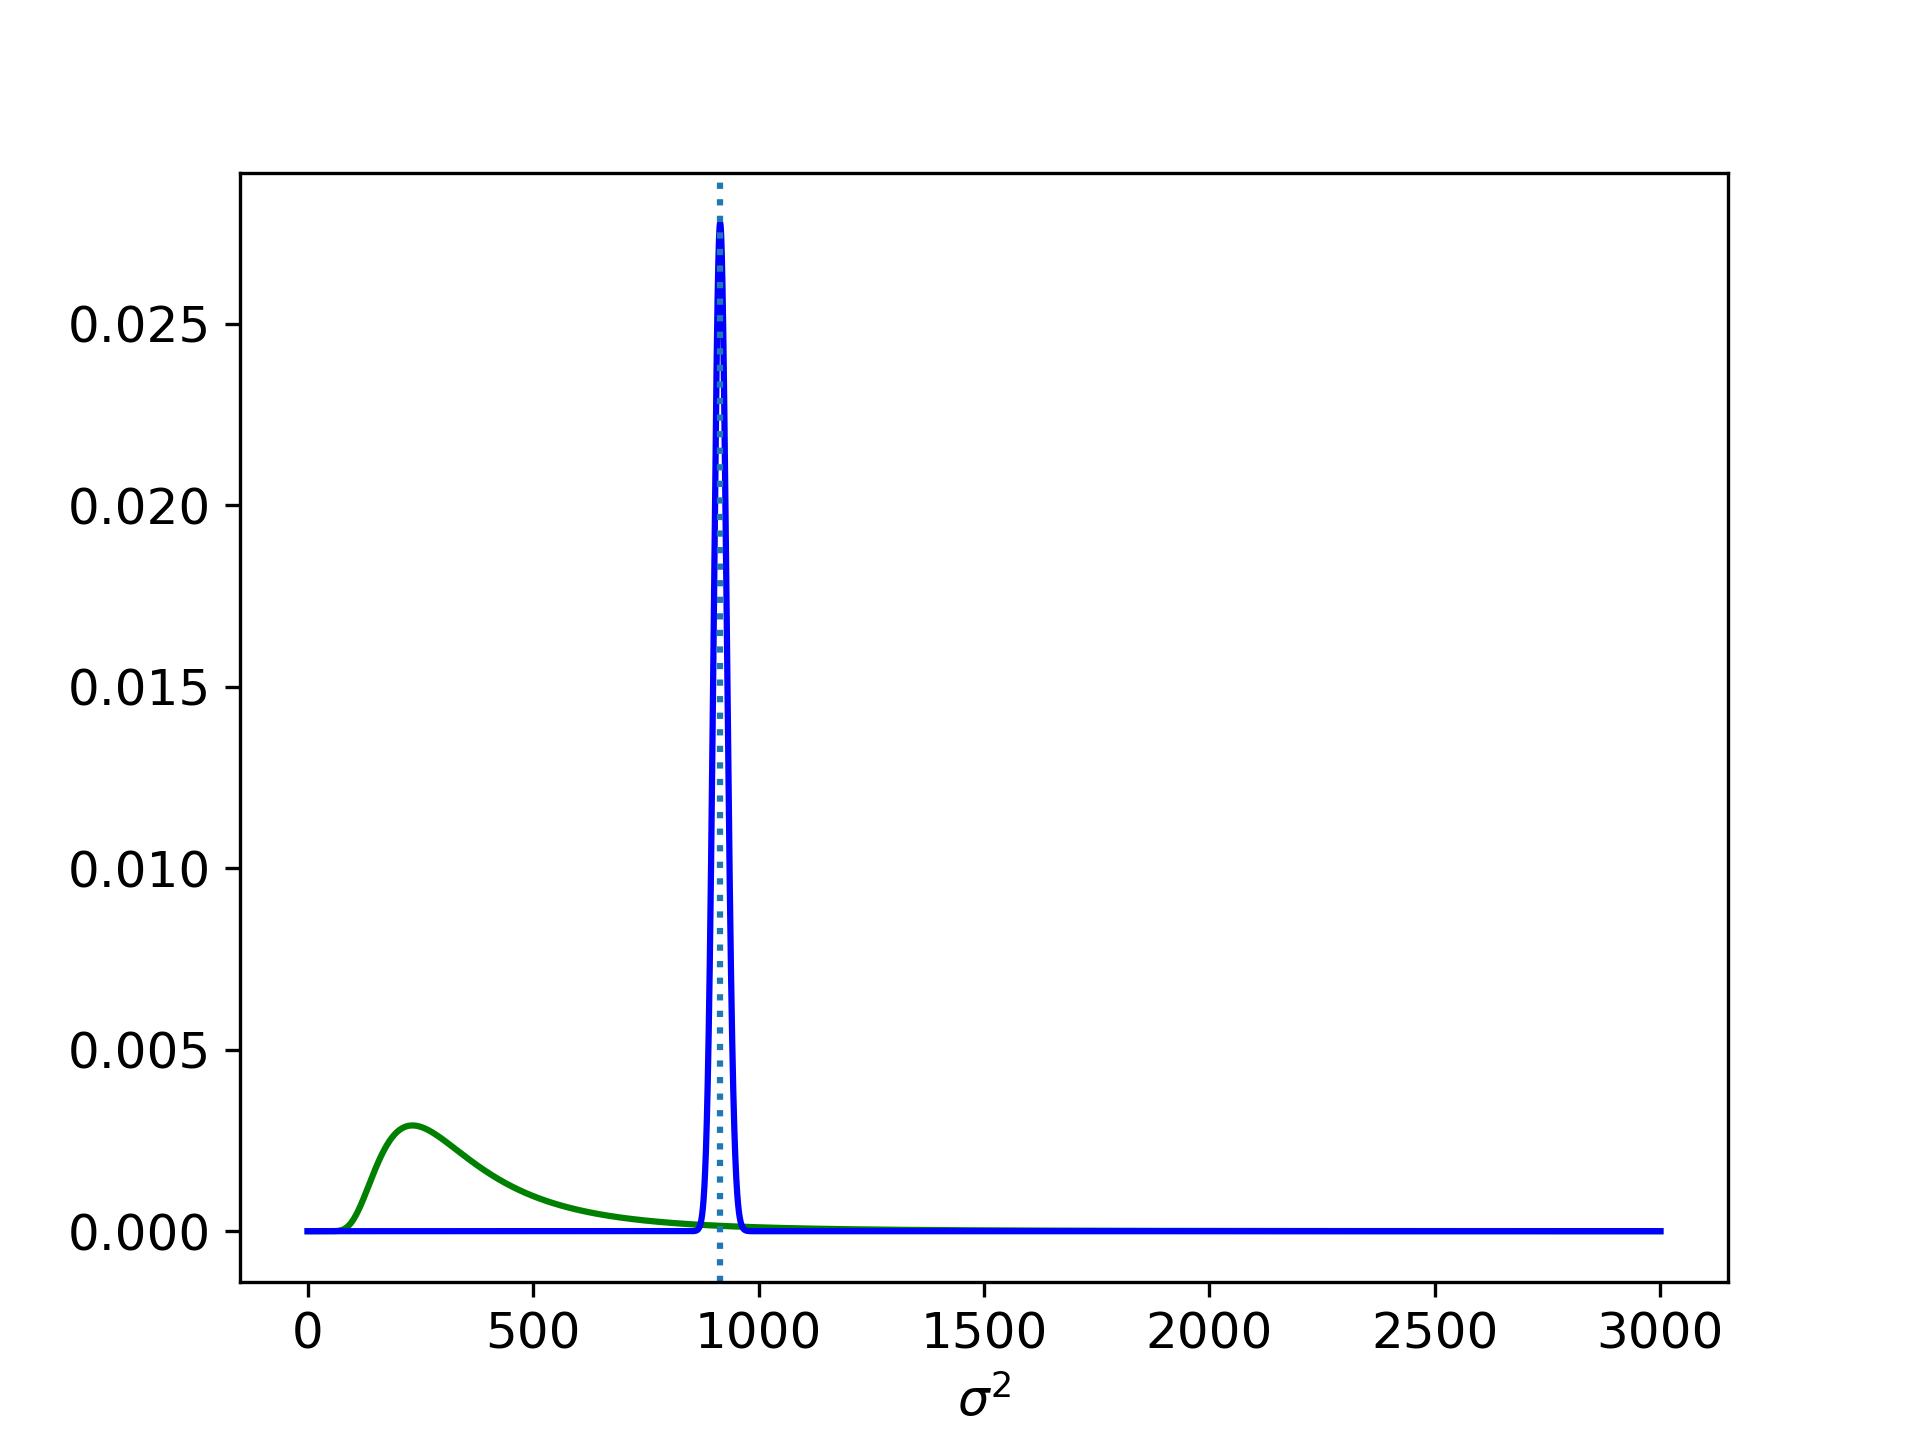
\includegraphics[scale=0.7]{3_3.png}

\end{document}
